\newpage
\sectiontitle{2.) Evidence of Eligibility to Apply}
\fakesection{Evidence of Eligibility to Apply}


%(A). Non-Tenured Faculty. Copy of Initial Employment Contract. The initial employment contract will indicate exactly when a candidate was first employed by the University and the years of prior service he or she has been granted. This information will allow the committee to verify the candidate’s eligibility for promotion and/or tenure. The copy of the initial contract of employment need not include the candidate’s salary.
%(B). Tenured Faculty. Evidence of Initial Date of Promotion (For faculty who have received a promotion and/or tenure at CSU): Document the effective date of the new rank by including the first contract at that rank. This documentation may include the letter from the University President stating the date the promotion was granted by the Board of Trustees as per Article 15.26 of the CSU-AAUP contract or a Personnel Action Form (PAF) that verifies the promotion.
%(C). Faculty not on tenure-track are not eligible for promotion or tenure.


\frame{
\textbf{Enclosed Files}

\begin{itemize}
\item Letter of Eligibility for Tenure -- Dated MONTH DAY, YEAR.
\item A copy of PAF, Dated MONTH DAY, YEAR.

\end{itemize}

}


\newpage


\includepdf[scale=0.9,pages=1-,pagecommand={}]{Files/2_Eligibility_letter/Eligibility_letter.pdf}
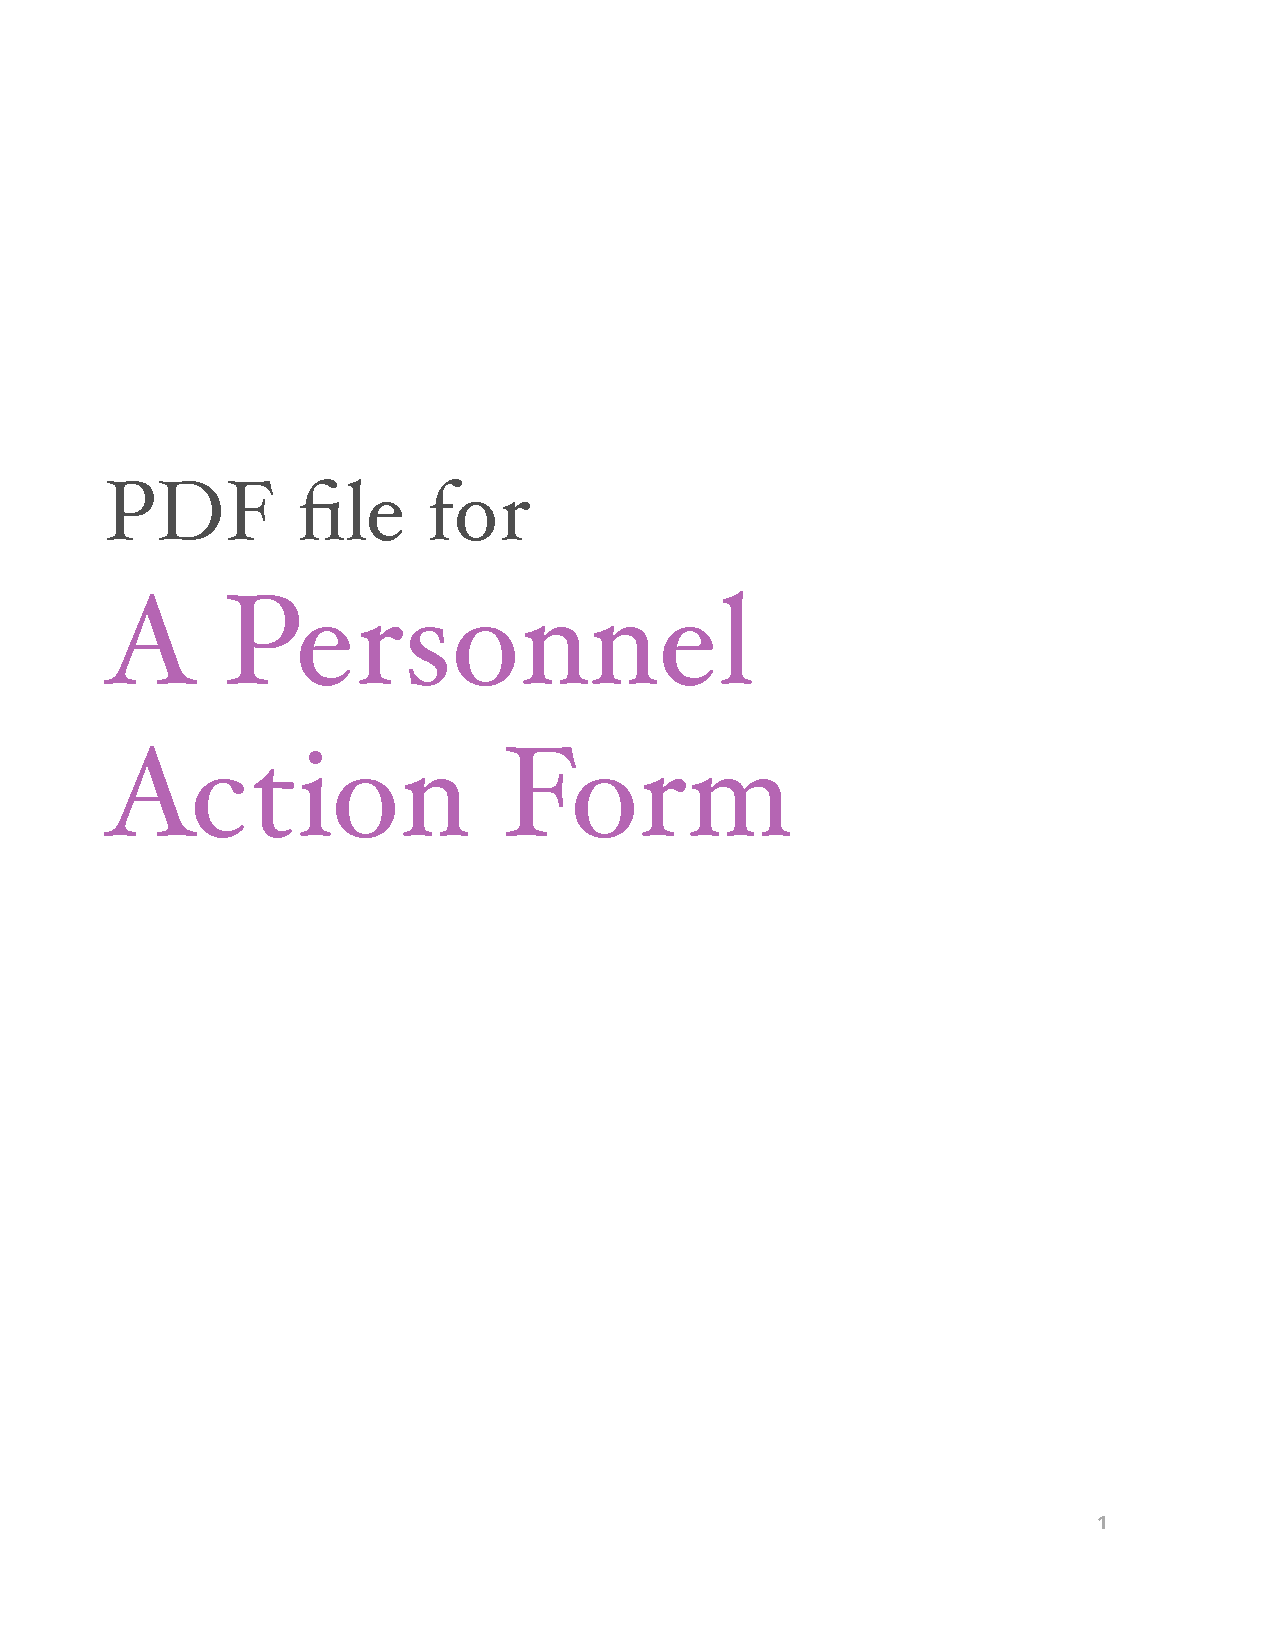
\includepdf[scale=0.9,pages=1-,pagecommand={}]{Files/2_Eligibility_letter/PAF.pdf}
